\begin{figure}[h]
\centering 
\includegraphics[scale=0.13]{images/Node.png}
\caption{Node.js logo}
\end{figure}
\noindent Node.js is a server-side platform built on Google Chrome's JavaScript Engine (V8 Engine). Node.js was developed by Ryan Dahl in 2009 and its latest version is v0.10.36.

Node.js is an open source, cross-platform runtime environment for developing server-side and networking applications. Node.js applications are written in JavaScript, and can be run within the Node.js runtime on OS X, Microsoft Windows, and Linux.

Node.js also provides a rich library of various JavaScript modules which simplifies the development of web applications using Node.js to a great extent.

\subsection{Features of Node.js}
\begin{itemize}
\item Asynchronous and Event Driven \− All APIs of Node.js library are asynchronous, that is, non-blocking. It essentially means a Node.js based server never waits for an API to return data.
\item Very Fast \− Being built on Google Chrome's V8 JavaScript Engine, Node.js library is very fast in code execution.
\item Single Threaded but Highly Scalable \− Node.js uses a single threaded model with event looping.
\item No Buffering \− Node.js applications never buffer any data. These applications simply output the data in chunks.
\end{itemize}
\subsection{Installation of Node.js}
Installation of Node.js is very easy. To install Node.js,
type the following commands:\\

	\$ curl -sL https://deb.nodesource.com/setup-6.x -o nodesource-setup.sh\\


	\$ nano nodesource-setup.sh\\


	\$ sudo apt-get install nodejs\\


	\$ sudo apt-get install build-essential\\


	\$ sudo apt-get install npm \\

\noindent This will install the node on your system.

\noindent \subsection{Creating Node.js project} The source code that you would write in a source file is simply javascript. The Node.js interpreter interprets and executes your javascript code.
\begin{itemize}
\item {\bf{Import Required Module}} We use the require directive to load the http module and store the returned HTTP instance into an http variable as follows −
\begin{figure}[h]
\centering 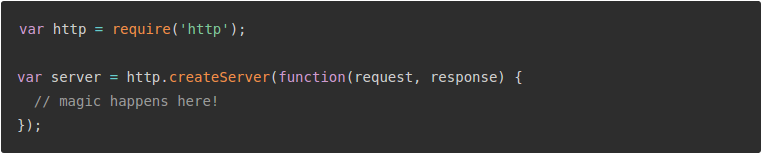
\includegraphics[scale=0.5]{images/1.png}
\caption{creating nodejs project.js}
\end{figure}

\item {\bf{Create Server}} We use the created http instance and call http.createServer() method to create a server instance and then we bind it at port 8081 using the listen method associated with the server instance. Pass it a function with parameters request and response. Write the sample implementation to always return "Hello World".
\begin{figure}[h]
\centering 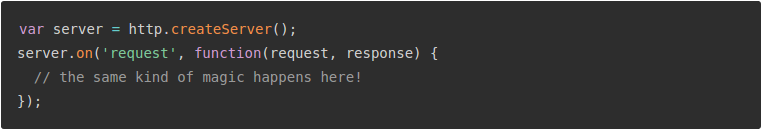
\includegraphics[scale=0.5]{images/2.png}
\caption{creating server.js}
\end{figure}

\item {\bf{Testing Request \& Response}} Let's put step 1 and 2 together in a file called main.js and start our HTTP server. Now execute the main.js to start the server as follows −

	\$ node main.js \\

\end{itemize}
\subsection{Starting Server in node.js}
In order to check your successful Node installation we can try out a very simple console command\\

	\$ node server.js \\

\noindent This command will start server in your console.\\

\subsection{Database setup}
To work with the database, you first need to create a connection. In this section of the tutorial, we will be using MongoDB’s native Node.js driver to create the connection with the MongoDB server. To install the mongodb native drivers, use the npm command to install the mongodb module. After that, run the following command in your project directory.

	\$ npm install mongodb \\

\begin{itemize}
\item npm is a package manager that provides a central repository for custom open source modules for Node.js and JavaScript. npm makes it simple to manage modules, their versions and distribution. As shown in the preceding paragraph, the npm install command was used to install the required module in our project.

\item Load the mongodb module : We used require to load the mongodb module in our code. mongodb module represents the native mongodb drivers for Node.js.

\item Defining the URL we need to connect to: We need to know where our mongodb server is running. The url represents the location where the mongodb server instance is running such that we can connect to it. The url contains the database name to which we intend to connect.

\item Connect to the database: Let’s use the MongoClient interface to connect to the database. In the callback we get error or the db object. We use the db object in order to communicate with the database.

\end{itemize}
